\documentclass[a4paper, 14pt]{extarticle}
\usepackage[T1]{fontenc}
\usepackage[utf8]{inputenc}
\usepackage[russian]{babel}
\usepackage[autostyle=true, style=russian]{csquotes}
\usepackage{amssymb,amsmath,color}
\usepackage{mathrsfs}
\usepackage{geometry}
%\geometry{a4paper, top=1.5cm, bottom=2.5cm, left=1.8cm, right=1.8cm}
\usepackage{graphicx}
\usepackage{indentfirst}
\usepackage[14pt]{extsizes}
\usepackage[export]{adjustbox}
\usepackage{siunitx}
\sisetup{output-decimal-marker = {,}}
\usepackage{float}
\usepackage{hyperref}
\usepackage{needspace}

\pagestyle{plain}
\textheight = 25cm %703pt % высота текста
\textwidth = 16cm %469pt % ширина текста
\oddsidemargin = 0.3cm % отступ от левого края
\evensidemargin = 0.3cm % отступ от левого края
\topmargin = -1.5cm %-40pt % отступ от верхнего края

\parindent=24pt
\setlength{\parskip}{1pt}
\widowpenalty=10000 % Висячие строки.
\clubpenalty=10000
\tolerance=1500 % терпимость к "жидким" строкам
\flushbottom % выравнивание высоты страниц
\linespread{1.1}% межстрочный интервал

\usepackage{enumitem}
\setlist[itemize]{
  itemsep=0.0em, parsep=0pt,
  topsep=0pt, partopsep=0pt,
  label={--}
  }
\setlist[enumerate]{
  itemsep=0.0em, parsep=0pt,
  topsep=0pt, partopsep=0pt
  }

\newtheorem{Df}{Опр.}
\newtheorem{Ex}{Пример}
\newtheorem{Nt}{Замечание}
\newtheorem{Pb}{Задача}
\newtheorem{Th}{Теорема}
\newtheorem{Lm}{Лемма}
\newtheorem{Ax}{Аксиома}

\def\dd#1#2{\frac{\partial#1}{\partial#2}} %частные производные.
\def\grad{\operatorname{grad}} %градиент.
\def\rang{\operatorname{rang}} %ранг.
\def\sign{\operatorname{sign}} %сигнум.
\def\abs{\operatorname{abs}} % abs.
\def\rot{\operatorname{rot}} % ротор.
\def\div{\operatorname{div}} % дивергенция.
\def\R{\mathbb{R}} % пространство R.
\def\Z{\mathbb{Z}} % пространство Z.
\def\Q{\mathbb{Q}} % пространство Q.
\def\N{\mathbb{N}} % пространство N.
\def\C{\mathbb{C}} % пространство C.
\def\inter{\operatorname{int}} %внутренность множества.
\def\intl{\int\limits} %интеграл, где область пишется под знаком интеграла.

\usepackage{caption}
\DeclareCaptionLabelSeparator{mydash}{~--~}
\captionsetup[figure]{
  name=Рисунок,
  labelsep=mydash,
  justification=centering,
  skip=0pt,
  aboveskip=12pt,
  belowskip=0pt
}
\captionsetup[table]{
  name=Таблица,
  labelsep=mydash,
  justification=raggedright,
  singlelinecheck=off,
  skip=0pt,  % Vertical space between block caption.
  aboveskip=0pt,
  belowskip=0pt
}

\usepackage{titlesec}
\newcommand{\nohyphens}{\hyphenpenalty=10000\exhyphenpenalty=10000}
% Chapter: size (pt), centered, numbered inline.
\titleformat{\section}
  {\normalfont\centering\bfseries\fontsize{14pt}{21pt}\selectfont\nohyphens}
  {\thesection}{6pt}{}  
\titleformat{name=\section,numberless}
  {\normalfont\centering\bfseries\fontsize{14pt}{21pt}\selectfont\nohyphens}
  {}{0pt}{}

  \makeatletter
\newcommand{\cyralph}[1]{%
  \ifcase#1\or А\or Б\or В\or Г\or Д\or Е\or Ж\or З\or И\or К\or Л\or М\or Н\or О\or П\or Р\or С\or Т\or У\or Ф\or Х\or Ц\or Ч\or Ш\or Щ\or Ъ\or Ы\or Ь\or Э\or Ю\or Я\else ??\fi}
\makeatother

\newcommand{\setupappendix}{%
    \setcounter{section}{0}% заменено на section для article
    \renewcommand{\thesection}{\cyralph{\value{section}}}%
    \renewcommand{\theHsection}{app\thesection}%
    \counterwithin{subsection}{section}%
    \counterwithin{figure}{section}%
    \counterwithin{table}{section}%
    \titleformat{\section}[display]
        {\normalfont\centering\bfseries\fontsize{14pt}{21pt}\selectfont}
        {}{0pt}{ПРИЛОЖЕНИЕ~\thesection\\}
    \titlespacing*{\section}{0pt}{0pt}{12pt}
}

\usepackage[sorting=none, backend=biber]{biblatex}
\setlength{\bibitemsep}{5pt}
\addbibresource{references.bib}

\graphicspath{{images/}}

\newcommand{\leftnohyphens}[1]{%
  {\raggedright\hyphenpenalty=10000\exhyphenpenalty=10000 #1\par}%
}

\begin{document}
    \thispagestyle{empty}	
    \fontsize{14pt}{21pt}\selectfont

    \vspace{20mm}

    \hfill
    \begin{minipage}[t][][t]{0.4\linewidth} % 0.4 -- доля относительно ширины документа
        \hfill\text{УДК 62-529:004.852}
    \end{minipage}

    \vspace{30mm}
    \begin{center}
        {\large Горбунов Роман Леонидович}
    \end{center}

    \vspace{5mm}
    \begin{center}
        {\bf \large Алгоритмы внутрисхемного измерения частотных характеристик и идентификации параметров вторичных источников электропитания
            \par}
        
        \vspace{10mm}
        {%\small
            Направление подготовки 27.04.03 -- Системный анализ и управление
        }
        
        \vspace{10mm}
        РЕФЕРАТ        
        диссертации на соискание степени магистра
    \end{center}

    \vfill
    \begin{center}
        {Санкт-Петербург -- 2026}
    \end{center}
    
    \newpage
    
    \fontsize{14pt}{14pt}\selectfont	
    \noindent Работа выполнена на базе факультета информационных технологий и программирования в федеральном государственном автономном образовательном учреждении высшего образования \enquote{Национальный исследовательский университет ИТМО}.
    \vspace{3mm}\\
    \textbf{Научный руководитель}:\\ 
    кандидат физико-математических наук, доцент (квалификационная категория \enquote{ординарный доцент}) ФГАОУ ВО \enquote{Национальный исследовательский университет ИТМО}\\ 
    \textbf{Бабушкин Максим Владимирович}
    \vspace{3mm}\\
    \textbf{Рецензент}:\par
    \leftnohyphens{кандидат технических наук, ведущий инженер-программист ООО~\enquote{НТЦ~ПРОТЕЙ}}
    \noindent \textbf{Калиновский Илья Андреевич}
    \vspace{10mm}\\
    Защита состоится 15~июня~2026~г. в 10:00 часов по адресу: г.~Санкт-Петербург, Ломоносова~9М, ауд.~1220
    \vspace{20mm}\\
    \noindent Реферат разослан 01~июня~2026~г.
    \vspace{3mm}\\
    \fontsize{14pt}{15pt}\selectfont Секретать ГЭК \hfill Матвеева Милена Вадиимовна

    \newpage
    \fontsize{14pt}{21pt}\selectfont

    {\bfseries \centering ОБЩАЯ ХАРАКТЕРИСТИКА РАБОТЫ\par}
    \vspace{10pt}

    \needspace{1\baselineskip}
    \noindent\textbf{Актуальность темы}\par
    Во вторичных источниках электропитания, регулируемых электроприводах и других технических устройствах с линейной системой автоматического регулирования процедуры отладки, настройки и контроля качества сопровождаются измерением частотных характеристик разомкнутого и замкнутого контура регулирования, объекта управления, канала обратной связи, регулятора. Измерения проводятся специализированным лабораторным оборудованием -- анализаторами цепей (Network Analyzers), подключаемым в разрыв штатных измерительных цепей системы управления.

    В тоже время, современные источники электропитания все чаще оснащаются программным управлением (real-time embedded control), что создает предпосылки для внутрисхемного измерения характеристик без специализированного измерительного оборудования. Результаты измерений могут использоваться для автоматизированного тестирования и контроля изделий в производственном цикле.

    \needspace{1\baselineskip}
    \noindent\textbf{Цель работы}\par
    Разработать алгоритмы внутрисхемного измерения частотных характеристик и идентификации параметров вторичных источников электропитания.

    \needspace{1\baselineskip}
    \noindent\textbf{Задачи работы}\par
    \begin{enumerate}
        \item Разработать алгоритмы внутрисхемного измерения частотных характеристик.
        \item Разработать алгоритмы идентификации параметров на основе измеренных частотных характеристик.
        \item Выполнить экспериментальную оценку показателей качества измерений и идентификации параметров.
    \end{enumerate}

    \needspace{1\baselineskip}
    \noindent\textbf{Положения, выносимые на защиту:}
    \begin{enumerate}
        \item Разработан алгоритм внутрисхемного измерения частотных характеристик, основанный на инжекции в систему синусоидальных сигналов с последовательной сменой частоты и амплитуды, обеспечивающий оптимальный размер измеряемых сигналов-откликов системы с целью уменьшения продолжительности измерений.

        \item Разработан алгоритм идентификации параметров линейного динамического звена по его частотной характеристике, основанный на архитектуре энкодера-декодера, обеспечивающей однократную генерацию узких бинарных масок, соответствующих координатам частот вещественных полюсов и нулей передаточной функции звена.
    \end{enumerate}

    \needspace{1\baselineskip}
    \noindent\textbf{Достоверность и обоснованность полученных результатов}\par
    Работоспособность разработанных алгоритма внутрисхемного измерения частотных характеристик и алгоритма идентификации параметров подтверждены в серии экспериментов по измерению частотных характеристик источника питания. Достигаемые качественные показатели оценены путем сравнения эталонных результатов с результатами измерения характеристик и идентификации по ним параметров (Приложение~\ref{appendix:bench}).

    \needspace{1\baselineskip}
    \noindent\textbf{Соответствие направлению подготовки}\par
    Работа соответствует направлению подготовки \enquote{27.04.03 -- Системный анализ и управление} согласно перечню общепрофессиональных и профессиональных компетенций, приведенному в Приложении~\ref{appendix:skills}.

    \needspace{1\baselineskip}
    \noindent\textbf{Апробация работы}\par
    Основные результаты работы представлены на следующих конференциях:
    \begin{enumerate}
        \item XIII Конгресс молодых ученых. 08-11~апреля~2024~г., ИТМО, г.~Санкт-Петербург.
        
        \item LIII научная и учебно-методическая конференция ИТМО. 29~января-02~февраля~2024~г., г.~Санкт-Петербург.
        \item Всероссийская научно-практическая конференция с международным участием «Искусственный интеллект: научные достижения и прикладные задачи». 04-05~декабря~2025~г., Югорский государственный университет, г.~Ханты-Мансийск.
    \end{enumerate}
    
    \needspace{2\baselineskip}
    \noindent\textbf{Личный вклад автора}\par
    Автором лично разработаны алгоритм внутрисхемного измерения частотных характеристик и алгоритм идентификации параметров линейного динамического звена по его частотной характеристике. Автором проведены эксперименты по оценке качественных показателей разработанных алгоритмов, спроектирована архитектура модели, сгенерирован синтетический набора данных для обучения модели и выполнено обучение.

    {\bfseries \centering КРАТКОЕ СОДЕРЖАНИЕ РАБОТЫ\par}
    \vspace{10pt}

    \textbf{Во введении} обоснована актуальность темы работы, представлены цель и задачи работы перечислены выносимые на защиту положения, обоснована достоверность и подчеркнута практическая значимость результатов работы, приведены сведения об апробации и реализации результатов работы, обозначен личный вклад автора, представлен краткий обзор структуры выпускной квалификационно работы.
    
    \needspace{2\baselineskip}
    \noindent\textbf{Первая глава «Обзор алгоритмов измерения частотных характеристик и идентификации параметров макромоделей физических объектов»}\par
    Рассмотрены широко применяемые сегодня алгоритмы измерения частотных характеристик. Алгоритмы основаны на возбуждении системы внешним периодическим воздействием и измерении установившихся откликов системы с последующим преобразованием откликов в комплексные коэффициенты передачи методами Фурье. Применяются как узкополосные, так широкополосные воздействия \cite{Zhang2025}.
    
    Идентификации параметров макромоделей физических объектов на основе измеренных частотных характеристик сегодня чаще всего выполняется итерационными алгоритмами, построенными на дробно-рациональной аппроксимации передаточной функции. В индустрии наиболее распространен алгоритм \enquote{Vector Fitting} \cite{triverio2019vector}. В системах высокого порядка с целью уменьшить количество итераций прорабатываются решения с предварительной генерацией начальных приближений искомых параметров с помощью сверточных нейронных сетей \cite{hua2023deep}.

    \needspace{2\baselineskip}
    \noindent\textbf{Вторая глава «Разработка алгоритмов внутрисхемного измерения частотных характеристик»}\par
    
    Рассматриваемая система аналого-цифрового преобразования и цифровой обработки сигналов с воздействием на объект управления посредством импульсной модуляции. Операции в системе выполняются циклически с постоянным периодом ${T_{d}}$, соответствующим базовой частоте дискретного регулирования ${f_{d} = 1 / T_{d}}$.

    В канал управления системы аддитивно инжектируется сигнал в виде дискретной последовательности моногармонического типа с частотой ${f^{(k)}_{z}}$ и амплитудой ${Z^{(k)}}$. Алгоритм измерения частотной характеристики звена системы основан на последовательной смене частоты и амплитуды в серии из $K$-измерений. Каждому $k$-му измерению, ${k \in \{1, \dots, K\}}$, соответствует пара параметров ${Z^{(k)}}$, ${T^{(k)}_{z}}$, следовательно, и набор откликов ${x^{(k)}[n]}$, ${y^{(k)}[n]}$, ${z^{(k)}[n]}$, а также коэффициентов ${X^{(k)}\left[l\right]}$, ${Y^{(k)}\left[l\right]}$ их разложения в ряд Фурье.

    Под частотной характеристикой понимается набор $K$-пар значений ${f^{(k)}_{z}}$, ${H^{(k)}}$, где в каждом $k$-ом измерении
    \begin{equation}\label{eqn:complexFreqResp}
        H^{(k)} = \cfrac{Y^{(k)}\left[L^{(k)}\right]}{X^{(k)}\left[L^{(k)}\right]} = \left| H^{(k)} \right| e^{j \angle H^{(k)}},
    \end{equation}
    ${L^{(k)} = {T^{(k)}_{h}} / {T^{(k)}_{z}}}$.

    Длительность измерительного окна (рисунок~\ref{fig:Th_var_N_var}):
    \begin{equation}\label{eqn:windowlength}
        T^{(k)}_{h} = L^{(k)} \mathord{\cdot} T^{(k)}_{z} = L^{(k)} \mathord{\cdot} R^{(k)} \mathord{\cdot} T_{d} = \underbrace{L^{(k)} \mathord{\cdot} Q^{(k)}}_{N^{(k)}} \mathord{\cdot} \underbrace{M^{(k)} \mathord{\cdot} T_d}_{T^{(k)}_{s}},
    \end{equation}
    где ${R^{(k)} \in \mathbb{R}}$ -- соотношение между периодом инжектируемого сигнала и периодом выполнения операций в системе, ${Q^{(k)} \in \mathbb{R}}$.

    Для каждой $k$-й частоты ${f_{z}}$ задача сведена к поиску наборов ${\mathbf{s}_{(p)} \in \mathbb{N}_{> 0}^3}$ целых чисел ${N, M, L}$, при которых обеспечивается частота ${f_{z(p)}}$ с заданной степенью приближения ${\Delta\epsilon^{*}_{f}}$ к ${f_{z}}$
    \begin{equation*}
        \left| f_{z(p)} - f_{z} \right| = \Delta\epsilon_{f(p)} < \Delta\epsilon^{*}_{f},
    \end{equation*}
    при ограничениях
    \begin{equation*}
        N_\text{min} \leq N_{(p)} \leq N_\text{max}, \quad M_{(p)} < \frac{R}{2}.
    \end{equation*}

    Оптимальным считается такой набор ${\mathbf{s}^{*}}$, в котором параметр ${N}$ минимален из всех ${\mathbf{s}_{(p)}}$, отвечающих условию ${\Delta\epsilon_{f(p)} < \Delta\epsilon^{*}_{f}}$. В случае, когда ни один набор параметров не удовлетворяет этому условию, оптимальным считается набор ${\mathbf{s}^{*}_{(p)}}$, соответствующий минимальному отклонению ${\Delta\epsilon_{f(p)}}$. Таким образом, минимум количества точек $N$ обеспечивает минимальную продолжительность измерения частотной характеристики.

    \needspace{6\baselineskip}
    \noindent\textbf{Третья глава «Разработка алгоритмов идентификации параметров макромоделей»}\par
    
    \textit{Кратко, о чем третья глава} \par

    \textbf{В заключении} кратко подводятся полученные результаты.

    \needspace{6\baselineskip}
    \noindent\textbf{Публикации по теме работы}
    \begin{itemize}
        \item[[A1]] \textbf{Горбунов~Р.Л.} Алгоритм внутрисхемного измерения частотных характеристик встраиваемых систем управления/ Севостьянов~Н.А., науч. рук. Бабушкин~М.В. // Сборник тезисов докладов конгресса молодых ученых, СПб,  08-11~апреля~2024~г. С.~99-100. (0,1 п.л./ 0,1 п.л.)
        
        \item[[A2]] Бабушкин~М.В. Идентификация параметров динамических звеньев встраиваемых систем управления/ Бабушкин~М.В., \textbf{Горбунов~Р.Л.} // Сборник трудов II Всероссийской научно-практической конференции с международным участием «Искусственный интеллект: научные достижения и прикладные задачи», Ханты-Мансийск, 04-05~декабря~2025~г. С.~6-11. (0,5 п.л./ 0,4 п.л.)
    \end{itemize}
    
    \printbibliography[heading=bibintoc, title={СПИСОК ЦИТИРУЕМОЙ ЛИТЕРАТУРЫ}]
   
    \setupappendix

    \clearpage
    \section{Общепрофессиональные и профессиональные компетенции направления подготовки \enquote{27.04.03 -- Системный анализ и управление}}\label{appendix:skills}
    Работа соответствует следующим компетенциям Федерального государственного образовательного стандарта направления подготовки \enquote{27.04.03 -- Системный анализ и управление}
    \begin{enumerate}
        \item ОПК-4. Способен осуществлять оценку эффективности технических систем методами системного анализа и управления.
        \item ОПК-6. Способен применять методы математического, функционального и системного анализа для решения задач моделирования, исследования и синтеза автоматического управления техническими объектами.
        \item ОПК-8. Способен формулировать содержательные и математические задачи исследований, выбирать методы исследований, системно анализировать, интерпретировать и представлять результаты исследований.
        \item ПК-4. Способен формировать технические задания и участвовать в разработке аппаратных и (или) программных средств, экспертно-аналитических систем поддержки принятия оптимальных решений.
    \end{enumerate}

    \clearpage
    \section{Результаты экспериментов}\label{appendix:bench}

    Перечень оборудования лабораторного стенда (рисунок~\ref{fig:bench}):
    \begin{enumerate}
        \item Макет источника питания 180~Вт -- 1~шт.
        \item Источник питания GW~INSTEK~GPC-3060D (2x30~В, 2x6~А) -- 1~шт.
        \item Нагрузка электронная АКИП 1380/1 (150~В, 30~А, 300~Вт) -- 1~шт.
        \item Измеритель частотных характеристик AP300 -- 1~шт.
        \item Осциллограф АКИП-4126/4A-X -- 1~шт.
        \item Мультиметр FLUKE 17B+ -- 1~шт.
    \end{enumerate}
    
    \begin{figure}[H]
        \centering
        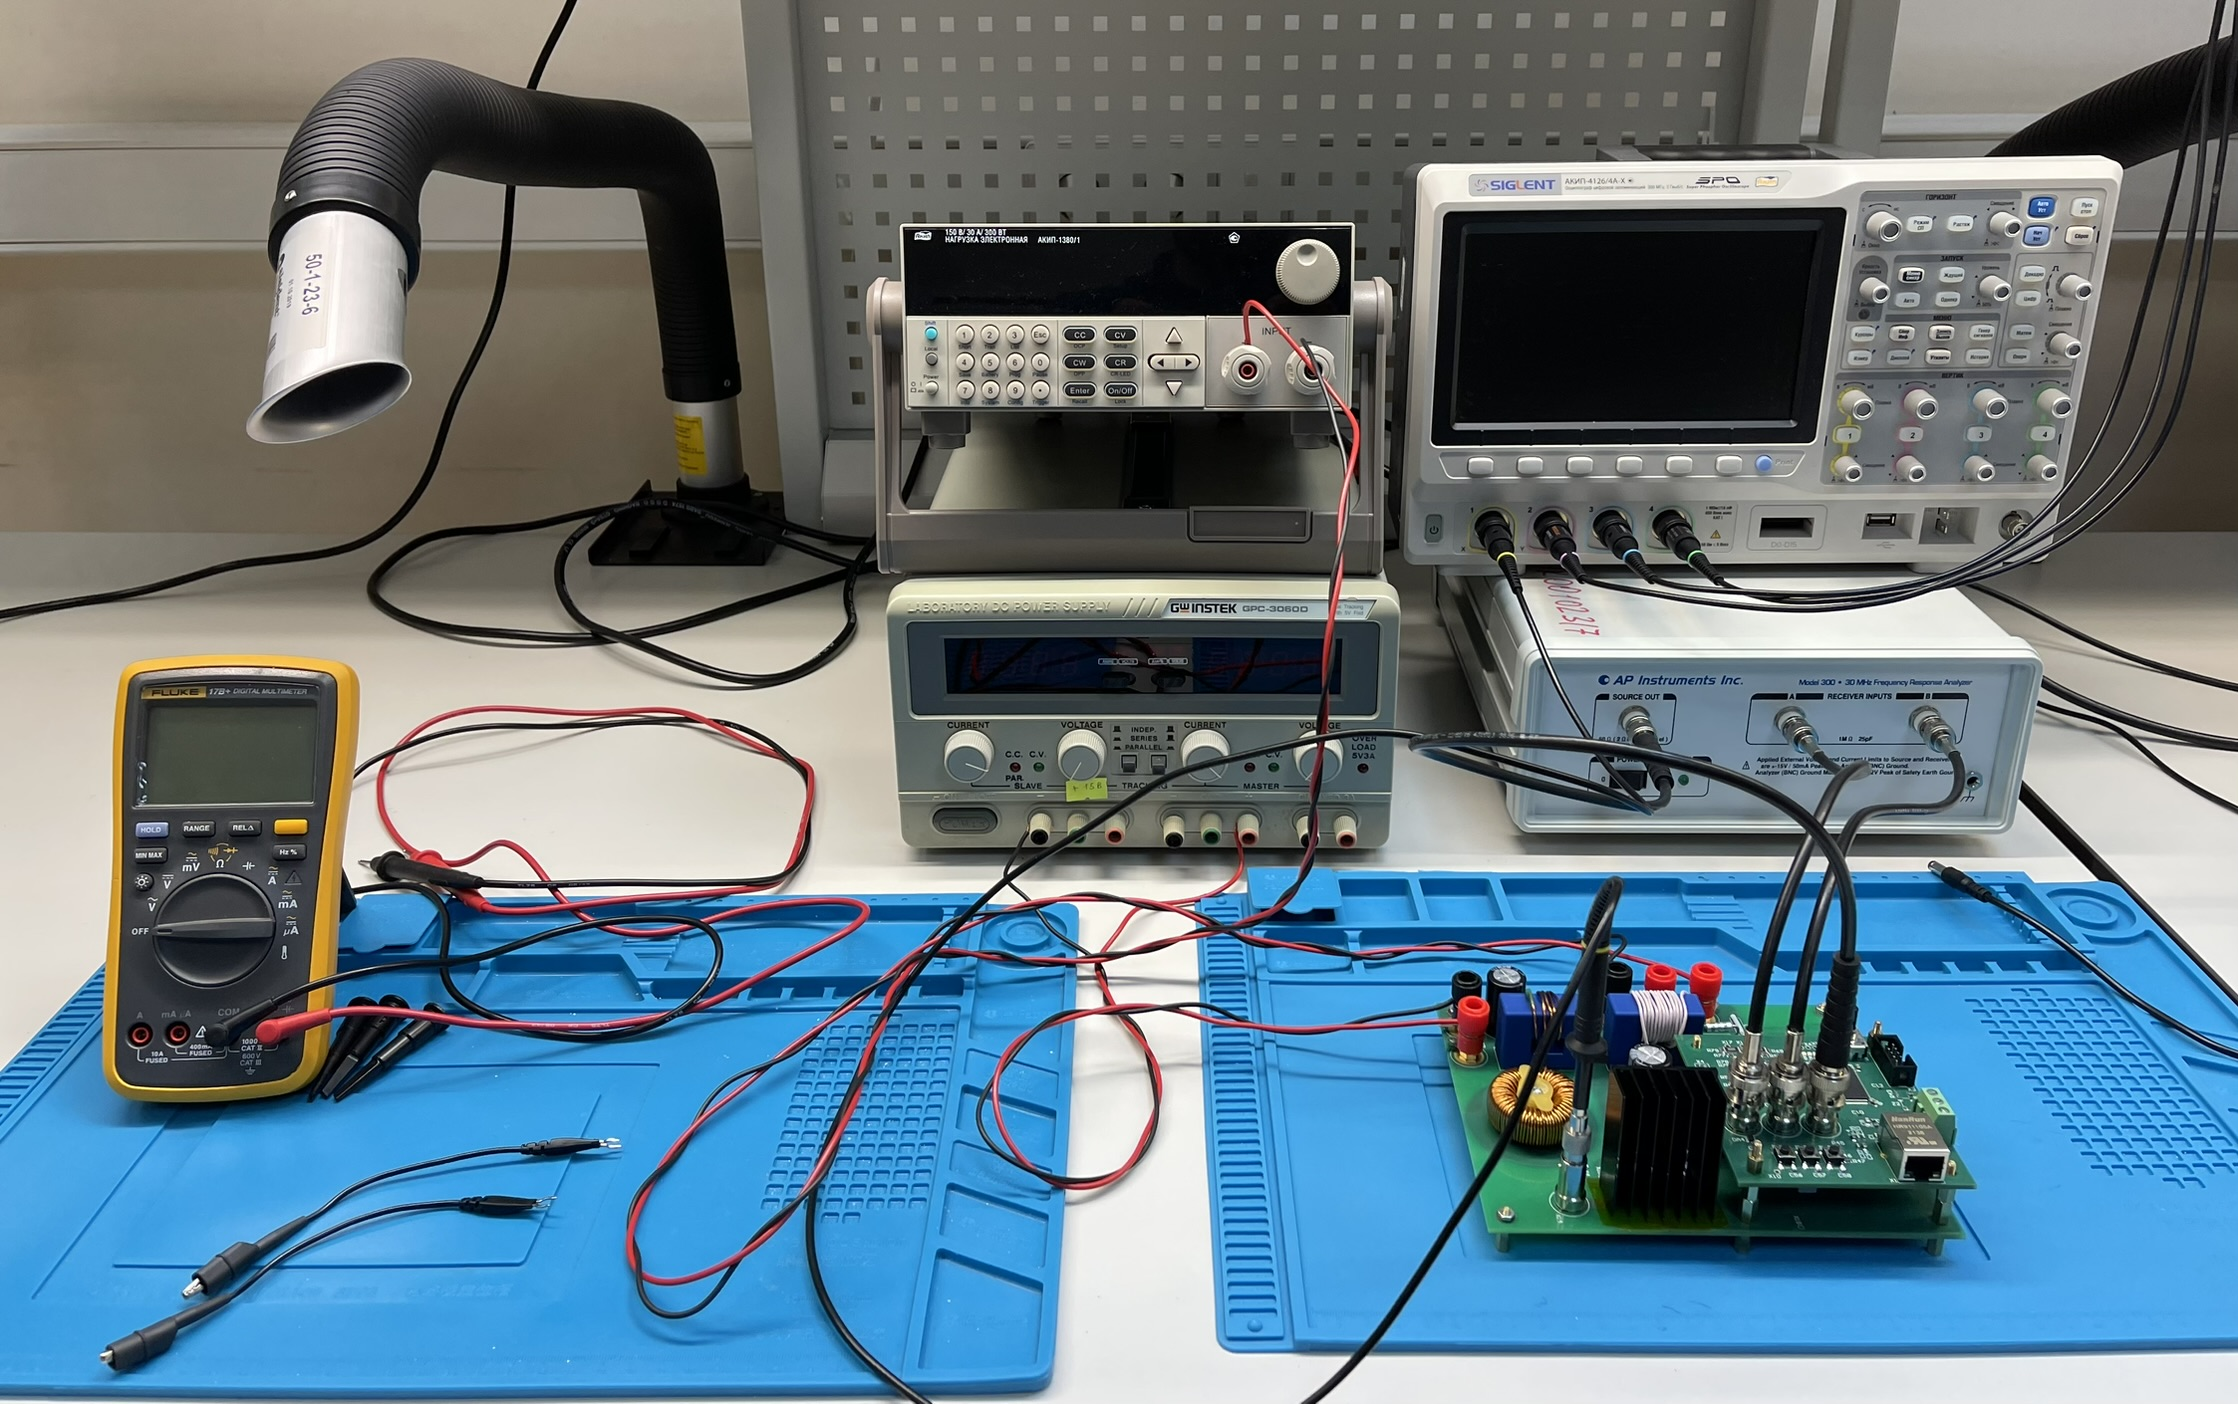
\includegraphics [width=1.00\linewidth] {appendix/bench.jpeg}

        \caption{Лабораторный стенд}
        \label{fig:bench}
    \end{figure}
    
    \clearpage
    \section{Алгоритм внутрисхемного измерения частотных характеристик}\label{appendix:freqresp}
    \begin{figure}[H]
        \centering
        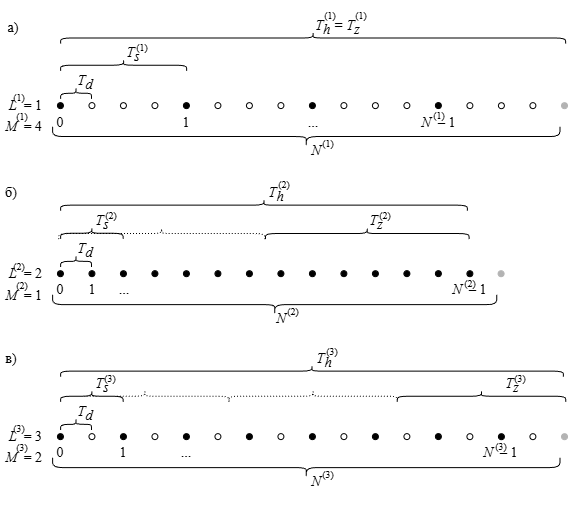
\includegraphics [width=1.00\linewidth] {frequencyResponse/Th_var_N_var.drawio.png}

        \caption{Параметры ${N, M, L}$ алгоритма при разных ${T^{(k)}_{z}}$}
        \label{fig:Th_var_N_var}
    \end{figure}
        
\end{document}